\documentclass[11pt,a4paper]{article}
\usepackage[margin=25mm,headheight=15pt]{geometry}
\usepackage[T1]{fontenc}
\usepackage{newtxtext}
\usepackage{mathtools,amsthm}
\usepackage{newtxmath}
\usepackage{microtype}
\usepackage{graphicx,booktabs,tabularx,longtable,array}
\usepackage{xcolor,enumitem,fancyhdr,titlesec}
\usepackage{xurl}
\usepackage[colorlinks=true,linkcolor=blue!35!black,citecolor=blue!35!black,urlcolor=blue!45!black]{hyperref}
\usepackage[nameinlink,noabbrev]{cleveref}
\hypersetup{pdftitle={Exponential Accuracy and Stokes Transport for Inverse Harmonic Transseries},pdfauthor={Research note prepared for Vladimir Reshetnikov},pdfsubject={Large-order asymptotics, certified inversion, and resurgence}}
\setlength{\parskip}{4pt}
\setlength{\parindent}{1.25em}
\setlength{\emergencystretch}{2em}
\allowdisplaybreaks[1]
\renewcommand{\topfraction}{0.9}
\renewcommand{\bottomfraction}{0.85}
\renewcommand{\textfraction}{0.05}
\pagestyle{fancy}
\fancyhf{}
\fancyhead[L]{\small Inverse harmonic transseries}
\fancyhead[R]{\small ProveIt research extension}
\fancyfoot[C]{\thepage}
\renewcommand{\headrulewidth}{0.3pt}
\titleformat{\section}{\Large\bfseries}{\thesection}{0.65em}{}
\titleformat{\subsection}{\large\bfseries}{\thesubsection}{0.65em}{}
\newtheorem{theorem}{Theorem}[section]
\newtheorem{lemma}[theorem]{Lemma}
\newtheorem{proposition}[theorem]{Proposition}
\newtheorem{corollary}[theorem]{Corollary}
\theoremstyle{definition}
\newtheorem{definition}[theorem]{Definition}
\newtheorem{remark}[theorem]{Remark}
\newtheorem{problem}{Research problem}
\numberwithin{equation}{section}
\newcommand{\dd}{\mathop{}\!\mathrm{d}}
\newcommand{\ii}{\mathrm{i}}
\newcommand{\ee}{\mathrm{e}}
\newcommand{\R}{\mathbb R}
\newcommand{\C}{\mathbb C}
\newcommand{\N}{\mathbb N}
\newcommand{\coef}[2]{[#1^{#2}]}
\newcommand{\Oh}{\mathcal O}
\newcommand{\Borel}{\mathcal B}
\newcommand{\eps}{\varepsilon}
\newcommand{\rising}[2]{(#1)_{#2}}
\newcommand{\repo}{\textit{ProveIt}}
\newcommand{\cformal}{\mathscr C}
\newcommand{\abs}[1]{\left|#1\right|}
\newcommand{\norm}[1]{\left\|#1\right\|}
\newcommand{\statusline}[2]{\noindent\textbf{#1.} #2\par}
\begin{document}
\begin{titlepage}
\vspace*{10mm}
\noindent{\large\scshape Transseries and rigorous asymptotic inversion}\par
\vspace{9mm}
\noindent{\huge\bfseries\raggedright Exponential Accuracy\\[1mm] and Stokes Transport for\\[1mm] Inverse Harmonic Transseries\par}
\vspace{6mm}
\noindent{\Large Large-order coefficients, exact-rational certificates,\newline and a convergent inverse jump expansion\par}
\vspace{10mm}
\noindent Research note prepared for Vladimir Reshetnikov\par
\noindent 29 September 2026\par
\vspace{9mm}
\hrule
\vspace{5mm}
\begin{abstract}
The \repo\ companion on combinatorial transseries gives every coefficient of the inverse harmonic function and proves a remainder at each fixed algebraic order. This article develops the missing large-order and exponentially accurate layers for that particular family. Writing
\[
 H(x)=\psi(x+1)+\gamma,\qquad X=\ee^{y-\gamma},\qquad
 H^{-1}(y)=W(X)-\tfrac12,
\]
we prove a finite formula for the complete large-order expansion of the coefficients of
$W(X)\sim X+\sum_{n\ge1}h_nX^{1-2n}$. In particular,
$h_n\sim2(-1)^n\Gamma(2n)/(2\pi)^{2n}$.
A general factorial-convolution theorem supplies the proof rather than a fit to computed coefficients.

An exact Fermi--Dirac integral yields signed forward remainders and rationally checkable inverse enclosures. If $u_M$ is the local inverse of the forward expansion truncated after $M$ terms, and $M-\pi X$ stays bounded, we prove the sharp law
$u_M-W(X)=(-1)^M\sqrt X\,\ee^{-2\pi X}(1+\Oh(X^{-1}))$, including its first correction and an all-orders construction. The exact Borel kernel also determines the forward Stokes jump. Transporting that jump through inversion gives an explicit convergent expansion of every inverse exponential sector. Known nonlinear resurgence theorems identify the formal inverse as a Borel-summable resurgent series. Exact symbolic checks, 190-digit experiments, and independent exact-rational enclosure checks accompany the proofs.
\end{abstract}
\vspace{4mm}
\noindent\textbf{Scope and status.} These are proved, explicitly scoped extensions of the inspected repository material, not a claim to have settled all of its transseries questions. Binet's formulas and general resurgence closure are existing results, credited below. Global priority for the specialized theorems has not been established. No new Lean formalization is claimed.
\vfill
\noindent\small Repository snapshot: \texttt{04e06e032dff1966513bfba316966d52db3646b4}.\par
\noindent\small Source, PDF, verification programs, exact certificates, and recorded outputs are included in the accompanying archive.
\end{titlepage}
\begingroup
\small
\setlength{\parskip}{0pt}
\tableofcontents
\endgroup
\newpage

\section{The research question and the repository boundary}
\label{sec:scope}

\subsection{Why this family is a useful test case}
A transseries calculation can answer several quite different questions. It can determine a formal coefficient, prove an asymptotic expansion to a fixed order, locate the least term of a divergent expansion, assign a sum to the expansion, or identify the exponentially small difference between two such sums. None of these steps should be silently substituted for another.

The harmonic inverse is particularly suitable for separating these tasks. Its coefficients have a compact exact formula, its forward function has an explicit integral representation, and its Borel singularities lie on an arithmetic lattice. Yet nonlinear inversion already changes the large-order coefficients and creates arbitrarily many exponential sectors. Thus it is a nontrivial example in which the formal, analytic, and computational layers can all be made explicit.

The inspected starting point is the companion volume
\emph{Combinatorial Transseries and Their Inverses: Gamma quotients, finite exponential sums, moment sectors, moving saddles, arithmetic sheets, and $q$-products} in the \repo\ repository \cite{repo}. Its theorem labelled
\texttt{t2:thm:harmonic-inverse} gives
\begin{equation}
 h_n=-\frac{1}{2n-1}\coef{z}{n}
       \exp\bigl((2n-1)\cformal(z)\bigr),
 \qquad
 \cformal(z)=-\sum_{j\ge1}\frac{B_{2j}(1/2)}{2j}z^j,
 \label{eq:repo-coeff}
\end{equation}
and a fixed-order inverse remainder. The same volume explicitly distinguishes such results from global resurgence or Borel summation. It also records that formal inversion cannot supply Stokes constants not already determined by the original function. The group's README describes the distinction between its formal-calculus, analytic-inversion, and Lean interfaces \cite{reporeadme}.

This article takes those distinctions seriously. We retain the repository's normalization and prove the additional statements needed in this one family. The result is a scoped answer to its summation and large-order gap, not a claim that every family in the companion has the same solution.

\subsection{What is established here}
The central results are as follows. \Cref{thm:endpoint} is a general endpoint-dominance theorem for coefficients of $\exp(N_n\cformal)$ when $N_n=\Oh(n)$ and the input has $\Gamma(2n)$ growth. \Cref{thm:late} applies it to obtain every large-order correction to $h_n$. \Cref{thm:cert} gives a completely explicit inverse certificate, and \cref{thm:optimal} determines the sharp error of an optimally scaled \emph{forward-truncation inverse}. \Cref{thm:resurgence,thm:stokes} identify the summation class and all inverse Stokes sectors.

There are three deliberate boundaries. First, the exponentially accurate approximation $u_M$ is not the direct partial sum $X+\sum_{n\le M}h_nX^{1-2n}$. We do not transfer a sharp error statement between them without proof. Second, a positive-real least-term error $\ee^{-2\pi X}$ is not a positive-real Stokes jump: the actual Borel singularities are imaginary. Third, the exact-rational computations below certify numerical enclosures but are not kernel-checked Lean proofs.

\subsection{Relation to existing work}
General asymptotic reversion is classical; the distinction between formal inversion and remainder control is discussed, for example, by Fabijonas and Olver \cite{fo}. Borinsky develops a powerful algebraic calculus for factorially divergent series and their inverses \cite{borinsky}. Our coefficient proof is self-contained and tailored to the growing multiplier $2n-1$ and the growth $\Gamma(2n)$; it should be read in that broader context, not as a claim that factorial asymptotics under inversion is a newly discovered subject.

For resurgence, the nonlinear closure results used here are Sauzin's: closure under convergent substitution and under composition/inversion at infinity, together with the corresponding Borel-summability statements \cite{sauzin}. Our contribution in that part is the explicit specialization to the centered harmonic inverse and the finite all-sector jump formula. A targeted literature search and repository inspection support this positioning, but are not an exhaustive priority investigation.

\section{Normalization and the formal inverse}
\label{sec:normalization}

Put
\begin{equation}
 F(w)=\psi(w+\tfrac12),\qquad
 C(w)=F(w)-\log w,\qquad
 F(W(X))=\log X.
 \label{eq:normalization}
\end{equation}
Initially $X\ge1$ and $w>0$ are real. Then
\begin{equation}
 H^{-1}(y)=W(\ee^{y-\gamma})-\tfrac12.
 \label{eq:h-inverse}
\end{equation}
The complex branches needed for Stokes analysis will be specified separately. We reserve $C(w)$ for an exact function and $\cformal(z)$ for a formal power series:
\begin{equation}
 C(w)\sim\cformal(w^{-2})=\sum_{j\ge1}c_jw^{-2j},\qquad
 c_j=-\frac{B_{2j}(1/2)}{2j}.
 \label{eq:c-coeff}
\end{equation}
Thus
\begin{equation}
 c_1=\frac1{24},\quad c_2=-\frac7{960},\quad
 c_3=\frac{31}{8064},\quad c_4=-\frac{127}{30720}.
 \label{eq:c-first}
\end{equation}
The relevant centered expansion follows from the classical gamma-function formulas \cite{dlmf}; a direct integral proof will be given in \cref{sec:integral}.

\begin{proposition}[Formal inverse and fixed-order meaning]
\label{prop:formal}
There is a unique formal Laurent series
\begin{equation}
 W(X)=X+\sum_{n\ge1}h_nX^{1-2n}
 \label{eq:wformal}
\end{equation}
satisfying $\log(W/X)+\cformal(W^{-2})=0$. Its coefficients are given by \eqref{eq:repo-coeff}. For every fixed $M\ge0$, the actual positive inverse satisfies
\begin{equation}
 W(X)=X+\sum_{n=1}^{M}h_nX^{1-2n}+\Oh(X^{-2M-1})
 \qquad (X\to+\infty).
 \label{eq:fixed-remainder}
\end{equation}
The constants in this assertion may depend on $M$.
\end{proposition}
\begin{proof}
Set $v=W^{-1}$ and $t=X^{-1}$. The formal equation becomes
$v=t\exp(\cformal(v^2))$. Formal Lagrange inversion gives a unique odd series $v(t)=t+\Oh(t^3)$. For $n\ge1$, its Laurent version gives
\[
 \coef{t}{2n-1}\frac1{v(t)}
 =-\frac1{2n-1}\coef{u}{2n}
       \exp\bigl((2n-1)\cformal(u^2)\bigr),
\]
which is \eqref{eq:repo-coeff}. This Laurent identity also follows directly by the change of variable $t=v\exp(-\cformal(v^2))$ in formal residues.

For fixed $M$, substitute the finite candidate into a sufficiently long finite expansion of $F$. Coefficient cancellation makes the forward residual $\Oh(X^{-2M-2})$. Near the candidate, $F'(w)\asymp X^{-1}$, so the mean value theorem gives \eqref{eq:fixed-remainder}. The integral bounds below justify both the finite expansion and this slope estimate independently of formal manipulations.
\end{proof}

The first coefficients, already present in the repository, are
\begin{equation}
 h_1=-\frac1{24},\quad h_2=\frac3{640},\quad
 h_3=-\frac{1525}{580608},\quad
 h_4=\frac{615881}{199065600},\quad
 h_5=-\frac{3058641}{504627200}.
 \label{eq:h-first}
\end{equation}
It is important that \eqref{eq:fixed-remainder} alone says nothing about choosing $M$ proportional to $X$. The next sections supply information uniform in that different regime, using a different approximation.

\section{A factorial endpoint-dominance theorem}
\label{sec:endpoint}

The coefficient extraction in \eqref{eq:repo-coeff} has a growing parameter. A product with one large index and several small indices is much larger than a balanced product, but the number of factors is not fixed in the exponential. Both facts must be controlled.

\begin{lemma}[Uniform factorial convolution]
\label{lem:convolution}
Let $b_j=\Gamma(2j)=(2j-1)!$ for $j\ge1$. For $n\ge2$,
\begin{equation}
 \sum_{j=1}^{n-1}b_jb_{n-j}\le3b_{n-1}.
 \label{eq:binary-convolution}
\end{equation}
Consequently, for $1\le\ell\le n$,
\begin{equation}
 \sum_{\substack{i_1+\cdots+i_\ell=n\\ i_r\ge1}}
       b_{i_1}\cdots b_{i_\ell}
 \le3^{\ell-1}b_{n-\ell+1}.
 \label{eq:multi-convolution}
\end{equation}
\end{lemma}
\begin{proof}
For $n\ge4$, the two endpoint terms in \eqref{eq:binary-convolution} contribute $2b_{n-1}$. Every remaining normalized term is
\[
 \frac{b_jb_{n-j}}{b_{n-1}}
   =\frac{2n-2}{\binom{2n-2}{2j-1}}
   \le\frac{2n-2}{\binom{2n-2}{3}}.
\]
Their sum is at most
$6(n-3)/((2n-3)(2n-4))\le1$. The cases $n=2,3$ are immediate. Induct on $\ell$, applying the binary bound to the final convolution, to obtain \eqref{eq:multi-convolution}.
\end{proof}

\begin{theorem}[Endpoint extraction with a growing exponential parameter]
\label{thm:endpoint}
Let $A,D,B>0$, and let $\cformal(z)=\sum_{j\ge1}c_jz^j$ be a complex formal series satisfying
\begin{equation}
 |c_j|\le A D^j\Gamma(2j)\qquad(j\ge1).
 \label{eq:factorial-bound}
\end{equation}
Let $0<N_n\le Bn$, and define
\[
 d_n=\frac1{N_n}\coef{z}{n}\exp(N_n\cformal(z)),\qquad
 E_k(N)=\coef{z}{k}\exp(N\cformal(z)).
\]
For every fixed integer $K\ge0$,
\begin{equation}
 d_n=\sum_{k=0}^{K}c_{n-k}E_k(N_n)
       +\Oh\!\left(D^n\Gamma(2n)n^{-K-1}\right).
 \label{eq:endpoint-theorem}
\end{equation}
The implied constant may depend on $A,D,B,K$, but not on $n$ or on the particular choices $N_n\le Bn$.
\end{theorem}
\begin{proof}
Write $N=N_n$. Expansion by the number of factors gives
\begin{equation}
 d_n=\sum_{\ell=1}^{n}\frac{N^{\ell-1}}{\ell!}
       \sum_{\substack{i_1+\cdots+i_\ell=n\\ i_r\ge1}}
          c_{i_1}\cdots c_{i_\ell}.
 \label{eq:by-length}
\end{equation}
Assume $n>2K$. A composition containing a part $n-k$ with $0\le k\le K$ has exactly one such part. Selecting it in the exponential, or selecting its position in \eqref{eq:by-length}, shows that its total contribution is exactly
$c_{n-k}E_k(N)$. Thus the displayed sum in \eqref{eq:endpoint-theorem} is exact for all compositions with one of those large parts. We bound the rest in two groups.

\emph{Many factors.} By \cref{lem:convolution}, the absolute contribution of length $\ell=t+1$ divided by $D^nb_n$ is at most
\begin{equation}
 A\frac{(3AN)^t}{(t+1)!}\frac{b_{n-t}}{b_n}.
 \label{eq:length-majorant}
\end{equation}
For $t\le n/2$, the $2t$ factors in $b_n/b_{n-t}$ are each at least $n$, so this is bounded by
$A(3AB/n)^t/(t+1)!$. Summing over $K+1\le t\le n/2$ gives $\Oh(n^{-K-1})$. For $t>n/2$,
\[
 \frac{b_{n-t}}{b_n}\le\frac{\Gamma(n)}{\Gamma(2n)}\le n^{-n}.
\]
Summing \eqref{eq:length-majorant} over this range gives at most
$A n^{-n}\exp(3ABn)$, smaller than every fixed negative power of $n$.

\emph{A bounded number of factors, but no sufficiently large part.}
Fix $2\le\ell\le K+1$. Every remaining composition has a largest part $j$ with
$n/\ell\le j\le n-K-1$. There are at most $\ell$ choices for its position. Applying \eqref{eq:multi-convolution} to the other $\ell-1$ parts bounds the unsigned factorial sum by
\begin{equation}
 \ell\,3^{\ell-2}
   \sum_{\lceil n/\ell\rceil\le j\le n-K-1}
       b_jb_{n-j-\ell+2}.
 \label{eq:bounded-length}
\end{equation}
The summand is log-convex in $j$, so its maximum is at an endpoint. At the right endpoint it equals
$b_{n-K-1}b_{K-\ell+3}$. At the left endpoint, Stirling's formula gives, relative to $b_n$, an exponentially small quantity times a fixed power of $n$: its exponential factor is
\[
 \exp\{-2n\mathcal H(1/\ell)\},\qquad
 \mathcal H(a)=-a\log a-(1-a)\log(1-a)>0.
\]
It is therefore $\Oh_K(b_{n-K-1})$ as well. There are at most $n$ summands in \eqref{eq:bounded-length}. After restoring $A^\ell D^nN^{\ell-1}/\ell!$ and dividing by $D^nb_n$, the bound is
\[
 \Oh_K\!\left(n^\ell\frac{b_{n-K-1}}{b_n}\right)
 =\Oh_K(n^{\ell-2K-2})=\Oh_K(n^{-K-1}).
\]
There are only finitely many such $\ell$. Length one has no omitted contribution. Combining the two groups proves the theorem.
\end{proof}

\begin{remark}
The argument is insensitive to signs or complex phases. It also does not assume convergence of $\cformal$. At any specified order $K$, it replaces a coefficient involving the entire prefix $c_1,\dots,c_n$ by $K+1$ large-index coefficients and finite polynomials in $c_1,\dots,c_K$. This is the mechanism behind the complete large-order expansion below.
\end{remark}

\section{The complete large-order expansion of the inverse coefficients}
\label{sec:late}

For $s>1$, write $\eta(s)=(1-2^{1-s})\zeta(s)$. The centered Bernoulli coefficients satisfy the exact identity
\begin{equation}
 c_n=2(-1)^{n+1}\frac{\Gamma(2n)}{(2\pi)^{2n}}\eta(2n).
 \label{eq:c-factorial}
\end{equation}
It also follows from the moment integral in \cref{sec:integral}. Notice that $\eta(2n)=1+\Oh(4^{-n})$.

\begin{theorem}[All orders of late-coefficient asymptotics]
\label{thm:late}
Let $h_n$ be defined by \eqref{eq:repo-coeff}. For fixed $K\ge0$, set
\begin{equation}
 \mathcal R_K(n)=\sum_{k=0}^{K}
  \frac{(-1)^k(2\pi)^{2k}E_k(2n-1)}
       {\prod_{r=1}^{2k}(2n-r)},\qquad
 E_k(N)=\coef{z}{k}\exp(N\cformal(z)),
 \label{eq:R-K}
\end{equation}
where the empty product is one. Then
\begin{equation}
 h_n=\frac{2(-1)^n\Gamma(2n)}{(2\pi)^{2n}}
       \left(\mathcal R_K(n)+\Oh(n^{-K-1})\right).
 \label{eq:late-all}
\end{equation}
In particular,
\begin{align}
 \frac{h_n(2\pi)^{2n}}{2(-1)^n\Gamma(2n)}
 ={}&1-\frac{\pi^2}{12n}
 +\frac{\pi^4/288-\pi^2/12}{n^2}\nonumber\\
 &+\frac{-\pi^6/10368-\pi^4/1440-\pi^2/12}{n^3}
 +\Oh(n^{-4}).
 \label{eq:late-first}
\end{align}
Every coefficient of the expansion in $1/n$ is a finite, effectively computable polynomial in $\pi^2$ with rational coefficients.
\end{theorem}
\begin{proof}
Use \cref{thm:endpoint} with $D=(2\pi)^{-2}$, any fixed upper bound for $2\eta(2j)$ as $A$, and $N_n=2n-1$. Since $h_n=-d_n$, it gives
\[
 h_n=-\sum_{k=0}^{K}c_{n-k}E_k(2n-1)
       +\Oh\!\left((2\pi)^{-2n}\Gamma(2n)n^{-K-1}\right).
\]
Divide by $2(-1)^n\Gamma(2n)/(2\pi)^{2n}$ and use \eqref{eq:c-factorial}. For each fixed $k$, the factor $\eta(2n-2k)$ differs from one exponentially little. The gamma quotient is precisely the reciprocal product in \eqref{eq:R-K}. This proves \eqref{eq:late-all}.

The polynomial $E_k(2n-1)$ has degree at most $k$ in $n$. Its contribution in \eqref{eq:R-K} is therefore $\Oh(n^{-k})$. Expanding the finite rational expression to the requested power of $1/n$ proves existence and computability of the complete expansion. The first three polynomials are
\[
 E_1(N)=Nc_1,\qquad
 E_2(N)=Nc_2+\tfrac12N^2c_1^2,\qquad
 E_3(N)=Nc_3+N^2c_1c_2+\tfrac16N^3c_1^3.
\]
Substitution and expansion give \eqref{eq:late-first}.
\end{proof}

\begin{corollary}[Divergence, exact Gevrey order, and least-term scale]
\label{cor:gevrey}
The series $\sum_{n\ge1}h_nz^n$ has radius of convergence zero and has exact Gevrey order two. The inverse displacement series
$\sum_{n\ge1}h_nX^{1-2n}$ has exact Gevrey order one in $X^{-1}$, and its ordinary Borel transform has radius of convergence exactly $2\pi$. Moreover, uniformly when $n-\pi X$ stays bounded,
\begin{equation}
 |h_n|X^{1-2n}=2\sqrt X\,\ee^{-2\pi X}
                  \left(1+\Oh(X^{-1})\right).
 \label{eq:least-term}
\end{equation}
In particular, the signs of $h_n$ are eventually $(-1)^n$.
\end{corollary}
\begin{proof}
The leading asymptotic in \cref{thm:late} proves eventual nonzero alternating sign and factorial growth. Stirling's formula identifies $\Gamma(2n)$, up to an exponential factor and a power of $n$, with $(n!)^2$. No smaller Gevrey order can dominate that growth.

Under the convention
$\Borel(X^{-m})=\xi^{m-1}/\Gamma(m)$, the coefficient of $\xi^{2n-2}$ in the Borel transform of the displacement is $h_n/\Gamma(2n-1)$. Its magnitude is asymptotic to $2(2n-1)/(2\pi)^{2n}$, proving the radius assertion by the root test. Finally, insert $n=\pi X+\Oh(1)$ in Stirling's formula for the leading term of \eqref{eq:late-all}; it gives \eqref{eq:least-term}.
\end{proof}

This result describes large-order coefficients. It does \emph{not}, by itself, prove that a direct inverse partial sum has error equal to its least term. Such an assertion requires additional analytic information; the next two sections obtain a sharp result for forward-truncation inverses instead.

\section{An exact integral and explicit inverse certificates}
\label{sec:integral}

\subsection{The centered Binet formula}
The half-integer centering has a useful analytic consequence: the Bose kernel in Binet's formula becomes a positive Fermi kernel. This gives more than the signs of the Bernoulli coefficients; it gives the sign and size of the exact remainder.

\begin{lemma}[Exact centered integral and signed remainders]
\label{lem:fermi}
For $w>0$,
\begin{equation}
 C(w)=2\int_0^\infty
       \frac{t\,\dd t}{(t^2+w^2)(\ee^{2\pi t}+1)}.
 \label{eq:fermi}
\end{equation}
Put $a_j=|c_j|$, and, for $M\ge0$, define
\begin{equation}
 P_M(w)=\log w+\sum_{j=1}^M c_jw^{-2j},\qquad
 E_M(w)=a_{M+1}w^{-2M-2}.
 \label{eq:PM}
\end{equation}
Then $R_M(w)=F(w)-P_M(w)$ has the exact representation
\begin{equation}
 R_M(w)=2(-1)^Mw^{-2M}
  \int_0^\infty\frac{t^{2M+1}\,\dd t}
       {(w^2+t^2)(\ee^{2\pi t}+1)},
 \label{eq:exact-remainder}
\end{equation}
and consequently
\begin{align}
 0&<(-1)^MR_M(w)<E_M(w),\label{eq:remainder-bound}\\
 |R'_M(w)|&\le\frac{2M+2}{w}|R_M(w)|
             <\frac{2M+2}{w}E_M(w).\label{eq:remainder-derivative}
\end{align}
\end{lemma}
\begin{proof}
The digamma duplication identity and Binet formula \cite[\S\S5.5, 5.9]{dlmf} give
\[
 \psi(w+\tfrac12)=2\psi(2w)-\psi(w)-2\log2,
 \qquad
 \psi(w)=\log w-\frac1{2w}
 -2\int_0^\infty\frac{t\,\dd t}{(t^2+w^2)(\ee^{2\pi t}-1)}.
\]
In the integral with argument $2w$, substitute $t=2s$. The elementary identity
\[
 \frac1{\ee^u-1}-\frac2{\ee^{2u}-1}=\frac1{\ee^u+1}
\]
then proves \eqref{eq:fermi}. Finite geometric expansion of $(w^2+t^2)^{-1}$ proves \eqref{eq:exact-remainder}, with
\begin{equation}
 a_j=2\int_0^\infty\frac{t^{2j-1}\,\dd t}{\ee^{2\pi t}+1}
     =\frac{2\Gamma(2j)}{(2\pi)^{2j}}\eta(2j).
 \label{eq:moment}
\end{equation}
For the last identity, expand the Fermi factor in its alternating exponential series and integrate. Absolute convergence of the resulting integrated series holds since $2j>1$. Thus the moments agree with the centered Bernoulli coefficients in \eqref{eq:c-factorial}.

Positivity of the integrand gives the sign. Replacing $(w^2+t^2)^{-1}$ by $w^{-2}$ gives the strict bound in \eqref{eq:remainder-bound}. Differentiating its positive integral representation, the factor $w^{-2M}$ contributes $2M/w$, and the denominator contributes at most $2/w$ relative to its integrand. This proves \eqref{eq:remainder-derivative}. All differentiations are dominated on compact positive $w$-intervals by an exponentially integrable function.
\end{proof}

\subsection{A bracket that works before computing any correction}
The trigamma series gives
\begin{equation}
 F'(w)=\sum_{k=0}^\infty(w+\tfrac12+k)^{-2}
       >\frac1{w+1/2}>0.
 \label{eq:slope}
\end{equation}
The strict inequality follows by comparison with the integral of the decreasing summand. In particular, the forward equation has at most one positive solution.

\begin{theorem}[Explicit inverse bracket and a posteriori certificate]
\label{thm:cert}
For $X\ge1$, put
\begin{equation}
 a=X-\frac1{12X},\quad I_X=[a,X],\quad
 d_X=\frac1{12X^2}-\frac1{24a^2},\quad
 \ell_X=\frac1{24X^2}-\frac7{960X^4}.
 \label{eq:bracket-data}
\end{equation}
Both $d_X$ and $\ell_X$ are positive. The equation $F(w)=\log X$ has a unique root $W(X)$ in $(a,X)$. For every $v\in I_X$ and every $M\ge0$,
\begin{equation}
 |v-W(X)|\le (X+\tfrac12)
 \left(\left|P_M(v)-\log X\right|+E_M(v)\right).
 \label{eq:residual-cert}
\end{equation}
Suppose, in addition, that
\begin{equation}
 E_M(a)<\min(d_X,\ell_X),\qquad
 \frac{(2M+2)E_M(a)}a<\frac1{X+1/2}.
 \label{eq:certificate-conditions}
\end{equation}
Then $P_M(u_M)=\log X$ has a unique root $u_M$ in $I_X$, and
\begin{equation}
 |u_M-W(X)|<(X+\tfrac12)E_M(a),\qquad
 \operatorname{sgn}(u_M-W(X))=(-1)^M.
 \label{eq:uM-cert}
\end{equation}
\end{theorem}
\begin{proof}
Since $a\ge11X/12$, the first two quantities in \eqref{eq:bracket-data} immediately give $d_X>0$; positivity of $\ell_X$ is also immediate for $X\ge1$. Applying \cref{lem:fermi} with $M=0$ gives
\[
 F(a)-\log X<\log(a/X)+\frac1{24a^2}
 \le-\frac1{12X^2}+\frac1{24a^2}=-d_X.
\]
The same lemma with $M=2$ gives $F(X)-\log X>\ell_X$. Continuity and \eqref{eq:slope} prove the existence and uniqueness of $W(X)$ in the open interval.

For $v\in I_X$, the mean value theorem and \eqref{eq:slope} imply
\[
 |v-W(X)|\le(X+\tfrac12)|F(v)-\log X|.
\]
Splitting $F=P_M+R_M$ proves \eqref{eq:residual-cert}.

Under \eqref{eq:certificate-conditions}, the endpoint signs persist when $F$ is replaced by $P_M$. Moreover, throughout $I_X$,
\[
 P'_M(w)=F'(w)-R'_M(w)
 >\frac1{X+1/2}-\frac{(2M+2)E_M(a)}a>0.
\]
Thus $u_M$ exists and is unique there. Applying the residual estimate at $u_M$ proves its error bound. Finally,
\[
 F(u_M)-F(W(X))=R_M(u_M),
\]
whose sign is $(-1)^M$. Strict monotonicity of $F$ proves the asserted sign of the inverse error.
\end{proof}

The uniqueness in this theorem is local to the specified interval. A high-degree truncated forward expression need not be globally monotone on the whole positive axis. The interval and slope conditions are therefore part of the result, not optional numerical details. Conversely, \eqref{eq:residual-cert} needs no monotonicity assumption on $P_M$ and applies to any proposed approximation in $I_X$.

\section{Sharp exponential accuracy of forward-truncation inversion}
\label{sec:optimal}

\subsection{The main error law}
The finite-order estimates above remain valid when the truncation order depends on the large parameter. Their exact integral representation makes it possible to analyze the important regime $M\asymp X$ without extrapolating a fixed-$M$ big-O constant.

\begin{theorem}[Sharp optimal-scale inverse error]
\label{thm:optimal}
Let $X\to+\infty$ and let $M=M(X)$ be a nonnegative integer such that $M-\pi X$ stays bounded. Define
\begin{equation}
 \sigma=M+1-\pi X.
 \label{eq:sigma}
\end{equation}
For all sufficiently large $X$, the root $u_M$ in \cref{thm:cert} exists. Uniformly for bounded $\sigma$,
\begin{align}
 u_M-W(X)
 ={}&(-1)^M\sqrt X\,\ee^{-2\pi X}
   \left(1+\frac{B_1(\sigma)}X+\Oh(X^{-2})\right),
 \label{eq:optimal-error}\\
 B_1(\sigma)
 ={}&\frac\pi{12}
     +\frac{2\sigma^2-3\sigma+7/12}{2\pi}.
 \label{eq:B1}
\end{align}
More generally, there are effectively computable polynomials $B_j(\sigma)$, of degree at most $2j$, with $B_0=1$, such that, for each fixed $J\ge1$,
\begin{equation}
 u_M-W(X)=(-1)^M\sqrt X\,\ee^{-2\pi X}
 \left(\sum_{j=0}^{J-1}\frac{B_j(\sigma)}{X^j}
              +\Oh_J(X^{-J})\right).
 \label{eq:optimal-all}
\end{equation}
The constants in the remainders may be chosen uniformly for $\sigma$ in any prescribed compact interval.
\end{theorem}

The leading constant in \eqref{eq:optimal-error} is one, whereas the magnitude of an inverse-series term in \eqref{eq:least-term} has leading constant two. These are statements about different objects; their difference is not a contradiction. The theorem identifies the actual error of the root of a truncated \emph{forward} equation.

\subsection{Concentration of the exact remainder}
\begin{lemma}[The transition at the least forward term]
\label{lem:gamma-remainder}
Let $n=M+1$, $b=2\pi w$, and $\tau=n-\pi w$. As $w\to+\infty$, uniformly for bounded $\tau$,
\begin{equation}
 R_M(w)=(-1)^Mw^{-1/2}\ee^{-2\pi w}
 \left(1+\frac{2\tau^2-3\tau+7/12}{2\pi w}
            +\Oh(w^{-2})\right).
 \label{eq:RM-asympt}
\end{equation}
There is a full expansion of the parenthesis in powers of $w^{-1}$ with polynomial coefficients in $\tau$.
\end{lemma}
\begin{proof}
In \eqref{eq:exact-remainder}, substitute $u=2\pi t$ and put $s=2n=b+2\tau$. If $U$ has the gamma density $u^{s-1}\ee^{-u}/\Gamma(s)$ on $u>0$, then
\begin{equation}
 R_M(w)=(-1)^M\frac{2\Gamma(s)}{b^s}
 \left\{\mathbb E\frac1{1+(U/b)^2}+\Oh(2^{-s})\right\}.
 \label{eq:gamma-expectation}
\end{equation}
Indeed, $0<\ee^{-u}-(\ee^u+1)^{-1}<\ee^{-2u}$ and the rational factor is at most one. The normalized error is bounded by $2^{-s}$ exactly.

For $f(v)=(1+v^2)^{-1}$, direct differentiation gives
\[
 f(1)=\tfrac12,\quad f'(1)=-\tfrac12,\quad
 f''(1)=\tfrac12,\quad f'''(1)=0.
\]
Since $s=b+2\tau$, the gamma moments give
\[
 \mathbb E(U/b-1)=\frac{2\tau}{b},\qquad
 \mathbb E(U/b-1)^2=\frac1b+\Oh(b^{-2}),\qquad
 \mathbb E(U/b-1)^4=\Oh(b^{-2}).
\]
The fourth derivative of $f$ is bounded on the positive real axis. Taylor's theorem therefore yields
\begin{equation}
 \mathbb Ef(U/b)=\frac12+\frac{1/4-\tau}{b}+\Oh(b^{-2}).
 \label{eq:gamma-first}
\end{equation}
Stirling's formula with bounded shift gives
\begin{equation}
 \frac{\Gamma(b+2\tau)}{b^{b+2\tau}}
 =\sqrt{2\pi}\,b^{-1/2}\ee^{-b}
 \left(1+\frac{2\tau^2-\tau+1/12}{b}+\Oh(b^{-2})\right).
 \label{eq:gamma-shift}
\end{equation}
Multiplication of \eqref{eq:gamma-first} and \eqref{eq:gamma-shift} in \eqref{eq:gamma-expectation} proves \eqref{eq:RM-asympt}.

For all orders, use Taylor's theorem through degree $2J-1$. Every derivative of $f$ is bounded on $[0,\infty)$, and the even centered gamma moment gives a remainder $\Oh(b^{-J})$, uniformly for bounded $\tau$. Every moment used in the finite Taylor polynomial is explicit:
\begin{equation}
 \mathbb E(U/b-1)^j
 =b^{-j}\sum_{\ell=0}^j
       \binom j\ell(-b)^{j-\ell}\rising{s}{\ell}.
 \label{eq:gamma-moments}
\end{equation}
For the other factor, the shifted logarithmic Stirling expansion is
\begin{equation}
 \log\frac{\Gamma(b+d)}{\sqrt{2\pi}\ee^{-b}b^{b+d-1/2}}
 \sim\sum_{r\ge1}\frac{(-1)^{r+1}B_{r+1}(d)}{r(r+1)b^r},
 \qquad d=2\tau.
 \label{eq:shifted-stirling}
\end{equation}
This classical expansion has a uniform fixed-order remainder for bounded $d$ \cite{dlmf}. Expanding its exponential and using \eqref{eq:gamma-moments} is a finite algorithm at every requested order. The coefficient at $b^{-j}$ has degree at most $2j$ in $\tau$. The exponentially small Fermi-to-gamma replacement affects none of these coefficients.
\end{proof}

\subsection{Transport from the forward remainder to the inverse error}
\begin{proof}[Proof of \cref{thm:optimal}]
For bounded $M-\pi X$, Stirling's formula in \eqref{eq:moment} gives
\[
 E_M(a)=\Oh(X^{-1/2}\ee^{-2\pi X}).
\]
Here $a=X-1/(12X)$, so replacing $X$ by $a$ changes this estimate by a bounded factor tending to one. The quantities $d_X,\ell_X$ are bounded below by positive constants times $X^{-2}$. Both conditions \eqref{eq:certificate-conditions} therefore hold for sufficiently large $X$.

Write $w=W(X)$ and $\delta=u_M-w$. The certificate first gives
$\delta=\Oh(\sqrt X\ee^{-2\pi X})$. The equation $P_M(u_M)=F(w)$ reads
\[
 0=F(w+\delta)-F(w)-R_M(w+\delta).
\]
On $I_X$, $F'(w)\asymp X^{-1}$, $F''(w)=\Oh(X^{-2})$, and \eqref{eq:remainder-derivative} gives
$R'_M=\Oh(X^{-1/2}\ee^{-2\pi X})$. Taylor's theorem, followed by division by $F'(w)$, proves
\begin{equation}
 \delta=\frac{R_M(w)}{F'(w)}
           +\Oh(X\ee^{-4\pi X}).
 \label{eq:linearized-exponential}
\end{equation}
This exponentially smaller error affects none of the coefficients in \eqref{eq:optimal-all}.

The fixed-order inverse expansion and the forward derivative give
\begin{equation}
 w=X-\frac1{24X}+\Oh(X^{-3}),\qquad
 \frac1{F'(w)}=w\left(1+\Oh(w^{-2})\right).
 \label{eq:center-transport}
\end{equation}
Thus $\tau=M+1-\pi w=\sigma+\pi/(24X)+\Oh(X^{-3})$ and
\[
 \sqrt w\,\ee^{-2\pi w}
 =\sqrt X\,\ee^{-2\pi X}
       \left(1+\frac\pi{12X}+\Oh(X^{-2})\right).
\]
Substitute \cref{lem:gamma-remainder} in \eqref{eq:linearized-exponential} and use these identities. This gives \eqref{eq:optimal-error} and \eqref{eq:B1}.

For any higher fixed order, take sufficiently many terms of the same expansions. The fixed-order expansion of $w$ is legitimate inside these finite Taylor calculations, because its omitted powers can be made arbitrarily small compared with the requested relative power of $X^{-1}$. Equations \eqref{eq:gamma-moments} and \eqref{eq:shifted-stirling}, the finite coefficient formula for $W$, and reciprocal series for $F'$ give an algorithm for every $B_j$. The degree bound $2j$ is preserved by these operations: the only dependence on $\sigma$ comes from the bounded shift in the gamma factor and its moments. This proves \eqref{eq:optimal-all}.
\end{proof}

\begin{remark}[What ``optimal-scale'' means]
The theorem applies to every integer choice with bounded $M-\pi X$, not only the unique best integer at a given $X$. Minimizing the first correction $B_1$ as a polynomial in a continuous $\sigma$ suggests $\sigma=3/4$, followed by a nearest-integer choice of $M$. This is an asymptotic guide, not a claim that it determines the exact minimizing integer for every $X$. The readily implemented choice $M=\lfloor\pi X\rfloor$ is covered uniformly by the theorem.
\end{remark}

\section{Exact-rational numerical certification}
\label{sec:rational}

\subsection{Removing the floating-point premise}
All the coefficients $c_j$ are rational. When $X$ and a candidate $v$ are rational, the sole nonrational term in the residual of $P_M$ is $\log(v/X)$. It can be enclosed by elementary rational arithmetic. For $r>0$, let $t=(r-1)/(r+1)$. Then $|t|<1$ and
\begin{align}
 \log r&=2\sum_{k=0}^{N-1}\frac{t^{2k+1}}{2k+1}+\rho_N,\label{eq:log-rational}\\
 |\rho_N|&\le\frac{2|t|^{2N+1}}{(2N+1)(1-t^2)}.
 \label{eq:log-rational-bound}
\end{align}
This follows by integrating the geometric expansion of $(1-t^2)^{-1}$, or directly by bounding the tail of the absolutely convergent arctangent-hyperbolic series. For rational $r$, both endpoints of this enclosure are rational.

Apply \eqref{eq:log-rational} with $r=v/X$ and add the exact rational sum $\sum_{j=1}^Mc_jv^{-2j}$. The signed remainder interval from \eqref{eq:remainder-bound} then gives an exact rational enclosure for $F(v)-\log X$. There are two independent ways to finish. One can apply the bound \eqref{eq:residual-cert}; alternatively, at two rational endpoints $v_-,v_+$ one can verify
\[
 F(v_-)<\log X<F(v_+).
\]
Strict monotonicity proves that the true inverse is enclosed. Both checks are implemented in the accompanying certificate program.

The floating-point calculation only proposes a useful candidate. It is not an assumption in the final sign comparisons: an inaccurate candidate would simply fail the exact checks. The proof of each exported interval consists of rational inequalities together with \cref{lem:fermi,thm:cert} and \eqref{eq:log-rational-bound}.

\subsection{A concrete certified interval}
At $X=10$, so that the exact target is $y=\gamma+\log10$, the program certifies
\begin{equation}
 \begin{split}
 9.495837994871258428840380076882531132
 &<H^{-1}(\gamma+\log10)\\
 &<9.495837994871258428840380083938321964.
 \end{split}
 \label{eq:exact-interval}
\end{equation}
Every displayed endpoint is an exact finite decimal, and the rounding was directed outwards. The two strict inequalities were checked with Python's exact \texttt{Fraction} arithmetic, using rational Bernoulli coefficients generated by SymPy. Thus \eqref{eq:exact-interval} is not an enclosure inferred from the number of displayed floating-point digits.

The file \path{verification/certificates.json} also records enclosures for $X=5,20,40$, the truncation orders, the numbers of logarithmic terms used, and the outcomes of both exact sign checks. The corresponding targets are exactly $\gamma+\log X$. To handle an independently prescribed arbitrary real $y$, one must also enclose $X=\ee^{y-\gamma}$, or work with a certified enclosure for $y-\gamma$ in the residual. Treating a rounded value of $X$ as exact would solve a slightly different problem.

\subsection{An implementation-level algorithm}
Choose a truncation order near $\pi X$, verify \eqref{eq:certificate-conditions}, and approximate the root of $P_M(v)=\log X$ inside $I_X$. Convert that approximation to a rational candidate. Increase the number of terms in \eqref{eq:log-rational} until the logarithmic uncertainty is safely below the analytic remainder. Use \eqref{eq:residual-cert} to obtain rational endpoints, and check their forward signs directly. A failed check calls for a wider interval or more arithmetic precision, not an unproved rounding rule.

This algorithm separates three error sources: root-finding error, logarithm-evaluation error, and the exact forward truncation remainder. For $v$ close to $X$, the logarithm argument is especially favorable: $t=\Oh(X^{-2})$, so only a modest number of rational logarithmic terms is required, even when the desired absolute enclosure is exponentially narrow.

\section{Borel summation and the resurgent inverse}
\label{sec:borel}

\subsection{The exact Borel kernel}
We use the ordinary Borel transform at infinity,
\[
 \Borel\left(\sum_{m\ge1}a_mw^{-m}\right)(\xi)
       =\sum_{m\ge1}\frac{a_m}{\Gamma(m)}\xi^{m-1}.
\]
A Gevrey-one series has a locally convergent transform. A series is called $1$-summable in direction $\theta$ when that transform continues to a neighborhood of the ray of angle $\theta$, has at most exponential growth there, and its directional Laplace integral exists for sufficiently large $w$ in the dual sector. A resurgent germ has analytic continuation along paths avoiding a specified discrete singular set; here the permitted set is an additive lattice. These definitions distinguish local Borel convergence from continuation and from summability.

\begin{proposition}[Borel kernel of the centered correction]
\label{prop:kernel}
The Borel transform of $\cformal(w^{-2})$ is
\begin{equation}
 \widehat C(\xi)=\frac1\xi-\frac1{2\sinh(\xi/2)}.
 \label{eq:borel-kernel}
\end{equation}
The origin is removable. The other singularities are simple poles at
$\omega_k=2\pi\ii k$, $k\in\mathbb Z\setminus\{0\}$, with
\begin{equation}
 \mathop{\rm Res}_{\xi=\omega_k}\widehat C(\xi)=(-1)^{k+1}.
 \label{eq:borel-residue}
\end{equation}
For $\Re w>0$,
\begin{equation}
 C(w)=\int_0^\infty\ee^{-w\xi}\widehat C(\xi)\,\dd\xi.
 \label{eq:borel-laplace}
\end{equation}
\end{proposition}
\begin{proof}
The Bernoulli generating function at $1/2$ is
\[
 \frac{\xi\ee^{\xi/2}}{\ee^\xi-1}
 =\frac\xi{2\sinh(\xi/2)}
 =\sum_{m\ge0}\frac{B_m(1/2)}{m!}\xi^m.
\]
Subtract the constant, divide by $-\xi$, and use the vanishing of the odd Bernoulli polynomials at $1/2$. The resulting coefficient of $\xi^{2j-1}$ is
$-B_{2j}(1/2)/(2j)!=c_j/\Gamma(2j)$, proving \eqref{eq:borel-kernel}. The derivative of $2\sinh(\xi/2)$ at $2\pi\ii k$ is $(-1)^k$, proving \eqref{eq:borel-residue}.

For the exact Laplace identity, use the classical digamma integral
\[
 \psi(z)=\int_0^\infty
 \left(\frac{\ee^{-t}}t-\frac{\ee^{-zt}}{1-\ee^{-t}}\right)\dd t
\]
and the integral for $\log w$ obtained by subtracting exponentials divided by $t$ \cite[\S5.9]{dlmf}. Subtracting the two formulas at $z=w+1/2$ gives \eqref{eq:borel-laplace}. The subtraction is made inside the integral: the apparent singularity at zero cancels. At infinity, $\Re w>0$ gives absolute convergence. This also proves directly that the formal correction has the stated positive-direction Borel sum.
\end{proof}

\subsection{Passing through nonlinear inversion}
\begin{theorem}[Resurgence and summation of the harmonic inverse]
\label{thm:resurgence}
Let $\Omega=2\pi\ii\mathbb Z$. The formal map
\begin{equation}
 \widetilde G(w)=w\exp\bigl(\cformal(w^{-2})\bigr)=w+\Oh(w^{-1})
 \label{eq:formal-G}
\end{equation}
and its formal compositional inverse
$\widetilde W(X)=X+\sum_{n\ge1}h_nX^{1-2n}$ are $\Omega$-resurgent maps tangent to the identity at infinity. They are $1$-summable in every direction other than the two imaginary Borel directions. Their directional sums are inverse maps wherever the corresponding local inverses are defined near infinity.

In the positive direction, the sum of $\widetilde W$ is the real branch $W(X)$ considered above, for sufficiently large $X$. It continues uniquely to that branch for all $X\ge1$.
\end{theorem}
\begin{proof}
The meromorphic function \eqref{eq:borel-kernel} continues outside $\Omega$, which is closed, discrete, and stable under addition. On every closed angular sector avoiding the imaginary rays, its growth at infinity is bounded by an exponential, in fact much more mildly. Thus the formal correction is $\Omega$-resurgent and $1$-summable in each nonsingular direction.

Apply the nonlinear closure theorems of Sauzin \cite[Theorems 3, 5 and $5'$]{sauzin}: convergent substitution preserves this resurgent class; maps tangent to the identity are closed under composition and inversion; and the corresponding statements hold for $1$-summability, with summation commuting with the operations. The hypotheses apply to the exponential in \eqref{eq:formal-G}, and then to its inverse. This proves the first assertions. Multiplication by $w$ only shifts the formal powers and introduces no new nonzero Borel singular locations.

In the positive direction, \eqref{eq:borel-laplace} identifies the sum of $\widetilde G$ as $G(w)=w\ee^{C(w)}=\ee^{F(w)}$. Its positive local inverse satisfies $F(w)=\log X$ and is therefore $W(X)$ by uniqueness in \cref{thm:cert}. The same monotonicity supplies its continuation along $X\ge1$.
\end{proof}

The statement about $\Omega$ is a containment and continuation statement. It does not say that every nonzero point of $\Omega$ must be an actual singularity on every continuation sheet of the inverse Borel transform. Conversely, \cref{cor:gevrey} proves independently that its initial Borel disk has radius exactly $2\pi$, so the inverse is not made convergent by cancellation of all its nearest singularities.

A general closure theorem establishes membership in a function class, not explicit Stokes data. Those data are accessible here because the original kernel and all its residues are known. We now transport them through inversion without introducing any undetermined constants.

\section{Every inverse Stokes sector, with a convergence theorem}
\label{sec:stokes}

\subsection{Orientation and the exact forward jump}
Consider the positive imaginary Borel ray. Let $C_-$ be the Laplace continuation along a ray with angle just below $\pi/2$, and let $C_+$ be the continuation along a ray just above $\pi/2$. The subscripts refer to these Borel-ray angles, not to signs of $\Im w$. Use compatible logarithm branches and write
\[
 F_\pm(w)=\log w+C_\pm(w).
\]
Their common region includes large $w$ in a closed sector strictly inside the lower half-plane. In this region put
\begin{equation}
 \lambda=2\pi\ii,\qquad q(w)=\ee^{-\lambda w},\qquad |q(w)|<1.
 \label{eq:lambda-q}
\end{equation}
The lower Borel contour directed outwards, followed by the upper contour directed inwards, has positive orientation around the enclosed poles. Hence \eqref{eq:borel-residue} gives
\begin{equation}
 F_-(w)-F_+(w)
 =2\pi\ii\sum_{k\ge1}(-1)^{k+1}\ee^{-2\pi\ii k w}
 =\frac{\lambda q(w)}{1+q(w)}.
 \label{eq:forward-jump}
\end{equation}
For a finite wedge this is the residue theorem. Its infinite limit is justified by exponential decay of the Laplace factor, using radii separated from the lattice poles. The final residue series converges absolutely for $|q(w)|<1$.

With the lower-angle continuation from the positive Borel direction, $F_-$ is the continuation of $\psi(w+1/2)$ from the right half-plane. Thus the numerical tests may evaluate
$F_+=\psi(w+1/2)-\lambda q/(1+q)$ directly. This convention also fixes every sign in the inverse formula below.

\subsection{The inverse transport formula}
Let $L$ be a target in a compatible logarithmic coordinate and let
\begin{equation}
 g(L)=F_+^{-1}(L),\qquad
 \widetilde g(L)=F_-^{-1}(L),\qquad
 p(L)=g'(L),\quad D=\frac{\dd}{\dd L},\quad
 q_0=\ee^{-\lambda g(L)}.
 \label{eq:stokes-notation}
\end{equation}
The inverse branches are the nearby branches asymptotic to $\ee^L$ in the specified sector. These are locally defined analytic inverses; no claim of global univalence on the entire complex plane is needed.

\begin{theorem}[Explicit, convergent inverse jump expansion]
\label{thm:stokes}
For sufficiently large $g(L)$ in any fixed closed sector strictly inside the lower half-plane,
\begin{equation}
 \widetilde g(L)-g(L)=\sum_{n\ge1}A_n(L)q_0^n,
 \label{eq:inverse-jump}
\end{equation}
where
\begin{equation}
 \boxed{\displaystyle
 A_n(L)=(-1)^n\sum_{m=1}^{n}
    \frac{\lambda^m}{m!}\binom{n-1}{m-1}
             (D-n\lambda p)^{m-1}p.}
 \label{eq:An}
\end{equation}
The power denotes repeated application of the differential operator to the function on its right; $p$ is not held constant.

There are constants $r,c>0$, independent of sufficiently large $w_0=g(L)$ in the chosen sector, such that the series in the auxiliary variable $z$ with coefficients $A_n(L)$ converges for $|z|<c/|w_0|$. In particular, if
\begin{equation}
 \eta_0=\frac{|w_0q_0|}{c}<1,
 \label{eq:eta0}
\end{equation}
then the tail after $N$ sectors obeys
\begin{equation}
 \left|\widetilde g-g-\sum_{n=1}^NA_nq_0^n\right|
 \le r\,\frac{\eta_0^{N+1}}{1-\eta_0}.
 \label{eq:stokes-tail}
\end{equation}
The condition \eqref{eq:eta0} holds automatically sufficiently far out in the specified sector.
\end{theorem}
\begin{proof}
We first identify the coefficients. For an analytic locally invertible $F_+$ and a perturbation $r_0(w)$, the inverse of $F_+(w)+t r_0(w)$ satisfies the classical inverse-perturbation identity
\begin{equation}
 w(L,t)=g(L)+\sum_{m\ge1}\frac{(-t)^m}{m!}
                D^{m-1}\left(p(L)r_0(g(L))^m\right).
 \label{eq:inverse-perturbation}
\end{equation}
For completeness, put $v=F_+(w)$, so that $v=L-t r_0(g(v))$ and $w=g(v)$. Apply the Lagrange--B\"urmann formula to this local equation for $v$, with observable $g$. It gives \eqref{eq:inverse-perturbation}. Thus the identity is a local analytic coefficient statement, independent of the particular special function.

In the present case, $r_0(w)=\lambda q(w)/(1+q(w))$. For each $m\ge1$,
\[
 r_0(g)^m=\lambda^m\sum_{n\ge m}
              (-1)^{n-m}\binom{n-1}{m-1}q_0^n.
\]
Moreover, $Dq_0=-\lambda p q_0$, so induction gives
\[
 D^{m-1}(p q_0^n)
       =q_0^n(D-n\lambda p)^{m-1}p.
\]
To make coefficient extraction independent of the exact coefficient functions, first replace $q(w)$ in the perturbation by $\eps q(w)$, keeping $F_+$ fixed. The coefficient of $\eps^n$ uses only $1\le m\le n$ in \eqref{eq:inverse-perturbation}. It is $A_n(L)q_0^n$, with $A_n$ given by \eqref{eq:An}. This argument is finite at each sector and does not assume that a rearrangement of two unbounded sums is valid.

To prove actual convergence and the tail bound, freeze $w_0=g(L)$ and introduce an independent variable $z$. Consider
\begin{equation}
 F_+(w_0+\delta)-F_+(w_0)
 +\frac{\lambda z\ee^{-\lambda\delta}}
        {1+z\ee^{-\lambda\delta}}=0.
 \label{eq:auxiliary-implicit}
\end{equation}
At $(\delta,z)=(0,0)$ its derivative in $\delta$ is $F'_+(w_0)\ne0$. The analytic implicit function theorem therefore gives an analytic solution $\delta(z)$ with $\delta(0)=0$. Its Taylor coefficients are the previously obtained $A_n$ by uniqueness of formal implicit solutions.

Here the convergence disk can be controlled uniformly. Choose a fixed small $r>0$. The sectorial expansion gives
\[
 F_+(w_0+\delta)-F_+(w_0)
       =\frac{\delta}{w_0}+\Oh(|w_0|^{-2})
       \quad (|\delta|=r),
\]
uniformly as $|w_0|\to\infty$ in the closed sector. Consequently its modulus on that circle is at least $r/(2|w_0|)$ for sufficiently large $w_0$, and it has precisely one zero inside. For $|z|\le c/|w_0|$, with fixed sufficiently small $c>0$, the rational perturbation in \eqref{eq:auxiliary-implicit} is bounded by $2|\lambda|\ee^{|\lambda|r}|z|<r/(2|w_0|)$; its denominator has no zero there. Rouch\'e's theorem gives exactly one root, counted with multiplicity, inside $|\delta|<r$. The root is simple and varies analytically with $z$. Thus $|\delta(z)|<r$ on the stated disk.

Cauchy's estimate, with radii tending to $c/|w_0|$, yields
$|A_n(L)|\le r(|w_0|/c)^n$. The geometric tail proves \eqref{eq:stokes-tail}. Substituting $z=q_0$ in \eqref{eq:auxiliary-implicit} recovers the exact equation $F_-(w_0+\delta)=L$, so the sum is the required inverse difference. Finally, $|q_0|=\exp(2\pi\Im w_0)$ decreases exponentially in the sector, whereas $|w_0|$ grows only algebraically. This proves the last assertion.
\end{proof}

\subsection{The first three nonlinear sectors}
Writing primes for derivatives with respect to $L$, \eqref{eq:An} gives
\begin{align}
 A_1={}&-\lambda p,\label{eq:A1}\\
 A_2={}&\lambda p+\frac{\lambda^2}{2}
                     (p'-2\lambda p^2),\label{eq:A2}\\
 A_3={}&-\lambda p-\lambda^2(p'-3\lambda p^2)
       -\frac{\lambda^3}{6}
                   (p''-9\lambda pp'+9\lambda^2p^3).
 \label{eq:A3}
\end{align}
For evaluating them directly from the forward branch, at $w_0=g(L)$ one has
\begin{equation}
 p=\frac1{F'_+(w_0)},\quad
 p'=-\frac{F''_+(w_0)}{F'_+(w_0)^3},\quad
 p''=\frac{3F''_+(w_0)^2-F'_+(w_0)F'''_+(w_0)}{F'_+(w_0)^5}.
 \label{eq:pderivs}
\end{equation}
The $p'$ and $p''$ terms are essential. Treating $p$ as a constant would erase part of the second sector and several terms of the third. Likewise, the factor $q(w_0+\delta)$ must be shifted during inversion; replacing it by $q(w_0)$ would lose the terms in $p^2$ and $p^3$.

The expansion is convergent in its outer exponential marker, with exact analytic coefficient functions $A_n(L)$. Replacing those functions by truncated asymptotic series introduces an additional, separate error. This is the same distinction between exact sector amplitudes and their formal expansions emphasized in the repository.

\subsection{Why the positive-real error is not a Stokes jump}
For positive real $X$, the quantity $\ee^{-2\pi\ii X}$ has modulus one, so \eqref{eq:inverse-jump} is not a small-sector expansion on that ray. There is no positive-real singularity in the Borel kernel \eqref{eq:borel-kernel}, and the positive-direction Borel sum is unambiguous. The real error $\ee^{-2\pi X}$ in \cref{thm:optimal} is governed by the distance $2\pi$ to the nearest complex Borel singularities and by optimal truncation; it is not a freely adjustable real exponential addition to $W$.

This distinction also explains why a formal inverse coefficient list alone could not have determined \eqref{eq:forward-jump}: its normalization comes from the exact forward function and its lateral continuations. Once that normalization is specified, all nonlinear inverse sectors follow from the finite formula \eqref{eq:An}.

\section{Reproducible checks and their logical status}
\label{sec:checks}

The accompanying scripts were run for this article. They use exact rational arithmetic for the finite coefficient calculations, SymPy for symbolic residual identities, and mpmath at 190 decimal digits for the analytic comparisons. The separate certificate program uses 200-digit arithmetic only to propose candidate roots and then checks all exported interval assertions with exact fractions. The distinction matters: the floating-point tables test the formulas, whereas the exact interval checks instantiate a proved certificate.

\subsection{Late coefficients}
Let
\[
 T_n=\frac{h_n(2\pi)^{2n}}{2(-1)^n\Gamma(2n)}.
\]
The $h_n$ in the following table were computed as exact rational numbers, not fitted from the asymptotic expression. The columns compare $T_n$ with the finite rational-in-$n$ expressions $\mathcal R_K$ in \eqref{eq:R-K}, rather than with their further expansions in $1/n$.

\begin{table}[!htb]
\centering\small
\begin{tabular}{rcccc}
\toprule
$n$ & $T_n$ & $|T_n-\mathcal R_1|$ & $|T_n-\mathcal R_3|$ & $|T_n-\mathcal R_5|$\\
\midrule
20  & $0.957519636599$ & $8.07375\cdot10^{-4}$ & $2.97309\cdot10^{-8}$ & $1.36284\cdot10^{-9}$\\
40  & $0.979119023315$ & $2.07922\cdot10^{-4}$ & $6.00223\cdot10^{-9}$ & $3.38346\cdot10^{-14}$\\
80  & $0.989641503387$ & $5.24785\cdot10^{-5}$ & $4.17995\cdot10^{-10}$ & $1.21710\cdot10^{-15}$\\
160 & $0.994840420773$ & $1.31694\cdot10^{-5}$ & $2.75099\cdot10^{-11}$ & $2.19491\cdot10^{-17}$\\
\bottomrule
\end{tabular}
\caption{Actual large-order coefficient checks. Theorem~\ref{thm:late}, not the finite table, proves the all-orders conclusion.}
\label{tab:late}
\end{table}

\subsection{The sharp inverse error}
For $M=\lfloor\pi X\rfloor$, the normalized error is
$Q_X=(-1)^M(u_M-W)/(\sqrt X\ee^{-2\pi X})$. The values below compare it with the first-correction prediction $1+B_1(\sigma)/X$.

\begin{table}[!htb]
\centering\small
\begin{tabular}{rrccc}
\toprule
$X$ & $M$ & $|u_M-W|$ & $Q_X$ & $1+B_1(\sigma)/X$\\
\midrule
5  & 15  & $5.33350\cdot10^{-14}$  & $1.050244866478$ & $1.048469941131$\\
10 & 31  & $1.66230\cdot10^{-27}$  & $1.019148786413$ & $1.018435404563$\\
20 & 62  & $1.20674\cdot10^{-54}$  & $1.014267790151$ & $1.014167761314$\\
40 & 125 & $4.50221\cdot10^{-109}$ & $1.005782589474$ & $1.005751752002$\\
\bottomrule
\end{tabular}
\caption{Actual checks of the leading constant and first correction in \cref{thm:optimal}.}
\label{tab:optimal}
\end{table}

For these four values, the analytic bound $(X+1/2)E_M(a)$ evaluates respectively to approximately
$1.24171\cdot10^{-13}$, $3.62340\cdot10^{-27}$,
$2.50333\cdot10^{-54}$, and $9.18334\cdot10^{-109}$.
These displayed decimal evaluations are floating-point diagnostics of an analytic bound. The exported intervals in \path{certificates.json}, by contrast, are checked by exact rational inequalities.

\begin{figure}[!htb]
\centering
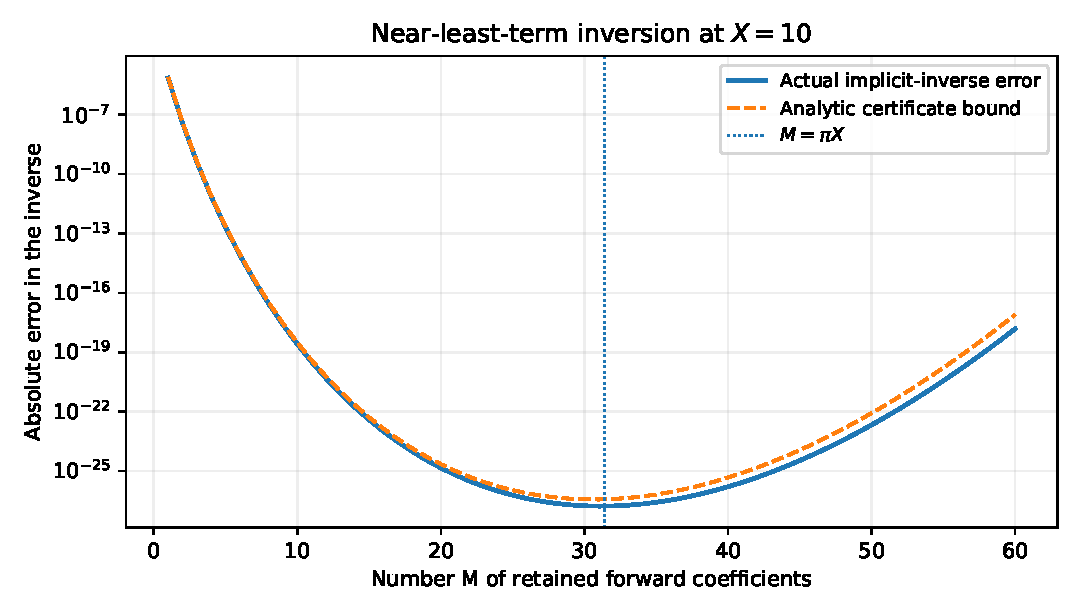
\includegraphics[width=\textwidth]{figures/optimal_truncation.pdf}
\caption{At $X=10$, increasing the number of retained forward coefficients first reduces and then increases the inverse error. The actual error is measured by high-precision root finding; the dashed curve evaluates the analytic bound from \cref{thm:cert}. The vertical line marks the scale $M=\pi X$, not an asserted exact integer minimizer.}
\label{fig:optimal}
\end{figure}

\subsection{Complex-sector checks}
The Stokes formula was tested by taking $w_0=2-\ii R$, setting
$F_+(w)=\psi(w+1/2)-\lambda q/(1+q)$, choosing $L=F_+(w_0)$, and solving the independent exact equation $\psi(w+1/2)=L$ near $w_0$. The first three coefficients were evaluated from \eqref{eq:pderivs}, not obtained by fitting that root.

\begin{table}[!htb]
\centering\small
\begin{tabular}{rcccc}
\toprule
$R$ & No sectors & Through $A_1q_0$ & Through $A_2q_0^2$ & Through $A_3q_0^3$\\
\midrule
2 & $6.19997\cdot10^{-5}$ & $2.38521\cdot10^{-8}$ & $1.37686\cdot10^{-11}$ & $9.42072\cdot10^{-15}$\\
3 & $1.47188\cdot10^{-7}$ & $1.34191\cdot10^{-13}$ & $1.83514\cdot10^{-19}$ & $2.97445\cdot10^{-25}$\\
\bottomrule
\end{tabular}
\caption{Absolute errors of successive inverse Stokes approximations.}
\label{tab:stokes}
\end{table}

The symbolic checks are logically separate. Substitution of the first six exact $h_n$ into the formal inverse equation cancels all residual coefficients through that order. Substitution of \cref{eq:A1,eq:A2,eq:A3} into a generic cubic Taylor model of \eqref{eq:auxiliary-implicit} cancels its first three powers of $z$ identically, with the forward derivatives treated as independent symbols. The exact Fermi integral was also compared numerically with the centered digamma function at $w=3/4,2,5$. All assertions in the supplied checks passed. None of these finite checks replaces the proofs for arbitrary order.

\section{Further research questions and concrete next steps}
\label{sec:questions}

The results isolate several sharply stated next problems. Their status here is ``not resolved in this article''; the list is not an assertion that every formulation has already been recognized as an open problem in the wider literature.

\begin{problem}[Direct inverse partial sums and an enveloping law]
\label{prob:direct}
For $S_M(X)=X+\sum_{n=1}^Mh_nX^{1-2n}$, determine whether a useful domain admits a signed first-omitted-term bound for $W(X)-S_M(X)$. In particular, determine the sharp remainder when $M-\pi X$ stays bounded.
\end{problem}
The forward expansion is enveloping by positivity of an exact Stieltjes-type integral. That property does not automatically survive nonlinear inversion. Theorem~\ref{thm:optimal} therefore cannot be reused as a proof for $S_M$. A promising route is to derive a contour representation for the inverse displacement itself and analyze the discontinuities of its continuation. Enveloping results for reverted Airy and cylinder-zero expansions, proved in a different setting by Nemes \cite{nemes}, show that an analytic inverse representation can be decisive. They do not settle the present function. A counterexample to a global sign claim would also be useful: it would specify the right local or asymptotic formulation before attempting a general theorem.

\begin{problem}[Explicit local singularities of the inverse Borel transform]
Determine the full local expansions of $\Borel(\widetilde W-X)$ at $\pm2\pi\ii$, including pole and logarithmic terms, and propagate them to subsequent lattice points on specified continuation sheets.
\end{problem}
The radius $2\pi$ and all inverse jump coefficients are already known here, but they do not constitute a complete description of local Borel singular germs on every sheet. The factorial asymptotics should constrain the nearest singular expansions, while \eqref{eq:An} supplies exact nonlinear consistency conditions. A constructive proof should match these two descriptions and state precisely which lattice points are actual singularities, rather than merely permitted singular locations.

\begin{problem}[A certified hyperasymptotic inverse]
Use the exact gamma-expectation remainder to improve $u_M$ beyond its entire first exponential block, with a rigorously quantified next exponential scale.
\end{problem}
Subtracting finitely many $B_j/X^j$ from \eqref{eq:optimal-all} improves the algebraic amplitude of $\ee^{-2\pi X}$; it does not by itself produce an error of order $\ee^{-4\pi X}$. To reach a second exponential layer, one must retain an exact or exponentially accurate first remainder block and then control both its own error and the quadratic inverse transport in \eqref{eq:linearized-exponential}. The exact expectation \eqref{eq:gamma-expectation}, together with a certified evaluation method for its rational gamma average, provides a concrete starting point.

\begin{problem}[Uniform passage from generalized harmonic inverses to the harmonic inverse]
Develop a uniform inversion and exponentially improved remainder theory for
$H_s(x)=\zeta(s)-\zeta(s,x+1)$ as $s\downarrow1$ and $x\to\infty$ jointly.
\end{problem}
The repository gives fixed-$s>1$ endpoint inverse coefficients in terms of
$T=((s-1)(\zeta(s)-y))^{-1/(s-1)}$. The singular normalization as $s\to1$ requires a renormalized target and control of the joint parameter $(s-1)\log x$. A useful theorem should recover the harmonic result in one limit and the fixed-$s$ endpoint result in another, with common remainder constants on an explicitly stated transition region. Merely substituting $s=1$ into a fixed-$s$ big-O estimate is insufficient.

\begin{problem}[Other inverse Bernoulli families and competing actions]
Apply the endpoint-extraction theorem to inverse gamma quotients and related exactly centered phases, then determine how several equally near complex actions interact under inversion.
\end{problem}
The proof of \cref{thm:endpoint} accommodates complex coefficients and does not require positivity. It can therefore extract late-coefficient contributions from several oscillatory factorial sources. What changes is the analytic normalization and the possibility of cancellation. A useful general result would identify when such cancellation changes the effective Gevrey scale or removes a nearest Borel singularity, and would connect those algebraic criteria to an exact remainder or contour representation for the original function.

\begin{problem}[Arithmetic action accumulation rather than a discrete Borel lattice]
Construct a summable inverse calculus for divisor-dependent sectors whose positive actions have a finite accumulation point, as in the repository's necklace and irreducible-polynomial examples.
\end{problem}
This is a separate frontier explicitly identified in the companion \cite{repo}. The lattice $2\pi\ii\mathbb Z$ used here is closed and discrete, so the standard nonlinear resurgence closure theorem applies. A divisor-action set accumulating at a finite location violates that hypothesis. Finite divisor cutoffs are well defined, but an infinite calculus must specify a topology or summability condition, retain the divisibility indicators, and justify products and inverse operations in that setting. A formal Hahn-support condition alone is not an analytic convergence argument.

\begin{problem}[Mechanization and bit complexity]
Formalize the finite factorial estimates and the exact-rational certificate first; then obtain an explicit bit-complexity bound for a certified inverse evaluation to a prescribed accuracy.
\end{problem}
The most accessible initial targets are \cref{lem:convolution}, the coefficient extraction underlying \cref{thm:endpoint}, the rational logarithm bound, and the mean-value enclosure in \cref{thm:cert}. They connect naturally to the repository's existing asymptotic-scale and backward-error interfaces \cite{reporeadme}. The full sectorial resurgence machinery is a much larger dependency and is not needed to certify positive-real values. The current scripts prioritize transparent arithmetic over optimal complexity; a faster implementation should use truncated-series algorithms and binary splitting for exact sums while preserving the same small certificate boundary.

\section{Synthesis}
\label{sec:synthesis}

For this specific inverse, the gap between formal transseries and quantitative analysis can be crossed completely along two complementary routes. On the positive axis, an exact positive integral yields signed remainders, explicit inverse brackets, and a sharp exponential error with all algebraic corrections. In the complex domain, an exact meromorphic Borel kernel fixes the forward jump, and a finite nonlinear coefficient formula transports it to a convergent inverse-sector expansion. Large-order coefficient asymptotics provide an independent connection between the two descriptions.

The logical dependencies remain visible. The all-coefficient inverse formula comes from the repository. The factorial endpoint estimate and its specialization prove the additional late-coefficient result. The exact centered integral is derived from classical Binet and duplication formulas. General resurgent closure is supplied by existing theory. The specific sharp inverse error and all-sector transport are then proved using those inputs. Exact-rational certificates turn the real error bounds into independently reproducible numerical enclosures. The next questions concern direct inverse truncation, finer Borel singular structure, higher exponential accuracy, uniform parameters, and action accumulation---not missing premises of the results proved here.

\appendix
\section{Finite coefficient algorithms}
\label{app:algorithms}

\subsection{Exact coefficients without expanding an exponential symbolically}
For fixed $N$ and degree $K$, set $E_0=1$ and use
\begin{equation}
 E_k=\frac Nk\sum_{j=1}^k j c_jE_{k-j},\qquad 1\le k\le K.
 \label{eq:E-recurrence}
\end{equation}
This is coefficient comparison in $(\exp(N\cformal))'=N\cformal'\exp(N\cformal)$. With $N=2n-1$ and $K=n$, it gives $h_n=-E_n/(2n-1)$ exactly. With $K$ fixed, it computes \eqref{eq:R-K} using only $c_1,\ldots,c_K$, regardless of the size of $n$. The current exact implementation takes quadratically many rational arithmetic operations for one such truncated exponential. The cost in bits also depends on the growth of numerator and denominator sizes.

For reference, the next two coefficients of the normalized late expansion after \eqref{eq:late-first}, with $p=\pi^2$, are
\begin{align}
 [n^{-4}]T_n={}&\frac{p^4}{497664}+\frac{p^3}{2880}
                   -\frac{37p^2}{1440}-\frac p{12},\label{eq:late-four}\\
 [n^{-5}]T_n={}&-\frac{p^5}{29859840}-\frac{23p^4}{1244160}
                   -\frac{403p^3}{362880}-\frac{29p^2}{288}-\frac p{12}.
 \label{eq:late-five}
\end{align}
Here the bracket notation denotes the coefficient in the asymptotic expansion in powers of $1/n$, not a power-series coefficient of a convergent function $T_n$.

\subsection{Computing a prescribed sharp-error coefficient}
To calculate $B_j$ in \eqref{eq:optimal-all}, take Taylor coefficients of $f(v)=(1+v^2)^{-1}$ at one through a sufficiently high even order. Replace powers of $v-1$ by the finite moment polynomial \eqref{eq:gamma-moments}, put $s=b+2\tau$, and expand to order $b^{-j}$. Multiply by the exponential of the finite shifted-Stirling series \eqref{eq:shifted-stirling}. Finally substitute $w=W(X)$ to the necessary finite order, use $\tau=\sigma+\pi(X-w)$, and multiply by $1/F'(w)$. At every fixed order this uses finitely many rational coefficients and powers of $\pi$.

The gamma-moment proof provides the error control for this algorithm. It is not merely a formal prescription for guessing $B_j$ from a numerical fit. Higher derivative estimates and central moments are needed only to the finite order requested.

\subsection{Computing inverse jump coefficients}
For each desired sector $n$, start with the function $p(L)$ and repeatedly apply $D-n\lambda p$ to obtain the $n$ expressions needed in \eqref{eq:An}. Combine them with the displayed finite binomial weights. This keeps the dependence on the exact dominant inverse visible and avoids expanding its internal asymptotic series prematurely. For evaluation, the derivatives of $p$ can instead be generated from derivatives of $F_+$ by implicit differentiation, as illustrated in \eqref{eq:pderivs}.

\section{Reproduction, provenance, and audit boundary}
\label{app:reproduction}

\subsection{Contents of the archive}
The archive contains this editable TeX source, its compiled PDF, the figure in PDF and PNG form, and three Python programs with their actual outputs. Run
\begin{verbatim}
python verification/verify.py
python verification/certify.py
python verification/make_figure.py
pdflatex -interaction=nonstopmode -halt-on-error \
  inverse_harmonic_transseries.tex
pdflatex -interaction=nonstopmode -halt-on-error \
  inverse_harmonic_transseries.tex
\end{verbatim}
The Python programs need Python 3.10 or later, SymPy, mpmath, and, for the figure, matplotlib. The PDF needs a normal LaTeX installation with the packages listed in the preamble, including \texttt{newtxtext} and \texttt{newtxmath}. No repository-relative style file is required. The stored figure permits rebuilding the article without rerunning the numerical computation.

\subsection{Exact repository checkpoint}
The inspection used commit
\begin{center}\small\texttt{04e06e032dff1966513bfba316966d52db3646b4}.\end{center}
The principal companion source is
\begin{quote}\small
\path{Analysis/FabiusFunction/docs/semi-formalized-research-frontiers/drafts/series-and-transseries/Combinatorial_Transseries_Inverses/Combinatorial_Transseries_Inverses.tex}.
\end{quote}
The relevant checkpoint source ranges were 4220--4500 for harmonic and generalized-harmonic inversion, 4500--4870 for certification and numerical distinctions, and 4870--5160 for support closure, status boundaries, and research questions. The group README and canonical transseries README were also inspected. These source ranges, paths, and commit identify a reproducible starting point; they are not a claim that every file in the repository was read.

\subsection{What the verification does and does not establish}
\statusline{Exact symbolic checks}{The displayed finite inverse and Stokes coefficients satisfy their defining residual identities through the checked orders.}
\statusline{Numerical checks}{The large-order, optimal-scale, integral, and complex-sector tests agree with the theorems at the recorded inputs and precision. These are finite floating-point tests, not universal proofs.}
\statusline{Exact-rational certificates}{The exported real inverse intervals have independently checked rational endpoint signs, using the proved analytic remainder inequality.}
\statusline{Human proofs}{The all-orders and uniform asymptotic statements are established in the arguments of the article, independently of the finite tests.}
\statusline{Not asserted}{No new Lean file is supplied; no global priority claim or complete treatment of all repository transseries families is made; and no sharp direct-inverse-partial-sum remainder is inferred from the forward-truncation theorem.}

\clearpage
\begin{thebibliography}{9}
\addcontentsline{toc}{section}{References}

\bibitem{repo}
Vladimir Reshetnikov, \emph{ProveIt}, companion manuscript
\emph{Combinatorial Transseries and Their Inverses: Gamma quotients, finite exponential sums, moment sectors, moving saddles, arithmetic sheets, and $q$-products}, repository snapshot
\texttt{04e06e032dff1966513bfba316966d52db3646b4}, inspected 29 September 2026. Exact path and inspected ranges in \cref{app:reproduction}.
\url{https://github.com/VladimirReshetnikov/ProveIt/tree/04e06e032dff1966513bfba316966d52db3646b4/Analysis/FabiusFunction/docs/semi-formalized-research-frontiers/drafts/series-and-transseries/Combinatorial_Transseries_Inverses}.

\bibitem{reporeadme}
Vladimir Reshetnikov, \emph{ProveIt}, ``Series and transseries'' group README and ``Transseries: the polynomial--logarithmic calculus and its inversions'' README, same snapshot.\newline
\url{https://github.com/VladimirReshetnikov/ProveIt/tree/04e06e032dff1966513bfba316966d52db3646b4/Analysis/FabiusFunction/docs/semi-formalized-research-frontiers/drafts/series-and-transseries}.

\bibitem{dlmf}
NIST Digital Library of Mathematical Functions, Chapter 5, especially \S5.5 (functional relations), \S5.9 (integral representations), and \S5.11 (asymptotic expansions), accessed 29 September 2026.
\url{https://dlmf.nist.gov/5.5};
\url{https://dlmf.nist.gov/5.9};
\url{https://dlmf.nist.gov/5.11}.

\bibitem{fo}
B. R. Fabijonas and F. W. J. Olver,
``On the reversion of an asymptotic expansion and the zeros of the Airy functions,''
\emph{SIAM Review} \textbf{41}(4) (1999), 762--773.
\url{https://doi.org/10.1137/S0036144598349538}.

\bibitem{borinsky}
M. Borinsky, ``Generating asymptotics for factorially divergent sequences,''
\emph{Electronic Journal of Combinatorics} \textbf{25}(4) (2018), P4.1.
\url{https://doi.org/10.37236/5999}.
Preprint: \url{https://arxiv.org/abs/1603.01236}.

\bibitem{sauzin}
D. Sauzin, ``Nonlinear analysis with resurgent functions,''
\emph{Annales scientifiques de l'\'Ecole normale sup\'erieure}, series 4,
\textbf{48}(3) (2015), 667--702.
\url{https://doi.org/10.24033/asens.2255}.
Preprint: \url{https://arxiv.org/abs/1212.4477}.

\bibitem{nemes}
G. Nemes, ``Proofs of two conjectures on the real zeros of the cylinder and Airy functions,''
\emph{SIAM Journal on Mathematical Analysis} \textbf{53}(4) (2021), 4328--4349.
\url{https://doi.org/10.1137/21M1396794}.
Preprint: \url{https://arxiv.org/abs/2010.13069}.

\end{thebibliography}
\end{document}
